\documentclass[ngerman]{gdb-aufgabenblatt}
\usepackage{enumitem}
\usepackage{dingbat}
\usepackage{ifsym}
\usepackage{amssymb}
\usepackage{amsmath}
\renewcommand{\Aufgabenblatt}{4}
\renewcommand{\Ausgabedatum}{Mi. 15.11.2017}
\renewcommand{\Abgabedatum}{Fr. 12.1.2018}
\renewcommand{\Gruppe}{Meimerstorf,Jochens,T�ter}
\renewcommand{\STiNEGruppe}{19}
\usepackage{tabularx}
\usepackage[normalem]{ulem}

\begin{document}

\section{Referentielle Aktion}
\begin{center}
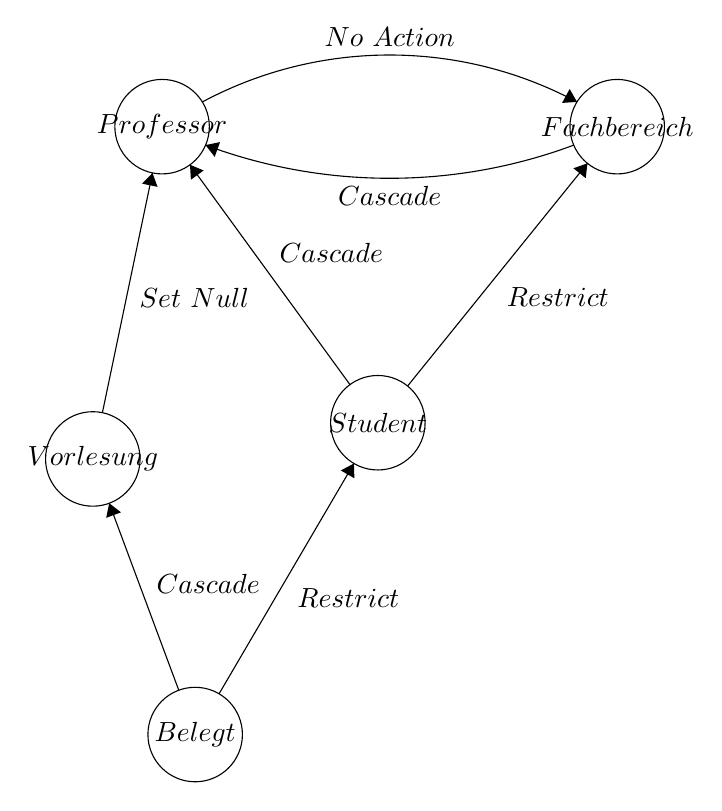
\begin{tikzpicture}[scale=0.2]
\tikzstyle{every node}+=[inner sep=0pt]
\draw [black] (10.1,-8.4) circle (3);
\draw (10.1,-8.4) node {$Professor$};
\draw [black] (23.8,-27.2) circle (3);
\draw (23.8,-27.2) node {$Student$};
\draw [black] (39,-8.4) circle (3);
\draw (39,-8.4) node {$Fachbereich$};
\draw [black] (5.7,-29.5) circle (3);
\draw (5.7,-29.5) node {$Vorlesung$};
\draw [black] (12.2,-47) circle (3);
\draw (12.2,-47) node {$Belegt$};
\draw [black] (22.03,-24.78) -- (11.87,-10.82);
\fill [black] (11.87,-10.82) -- (11.93,-11.77) -- (12.74,-11.18);
\draw (17.53,-16.42) node [right] {$Cascade$};
\draw [black] (12.655,-6.831) arc (118.14753:61.85247:25.215);
\fill [black] (36.45,-6.83) -- (35.98,-6.01) -- (35.5,-6.89);
\draw (24.55,-3.35) node [above] {$No\mbox{ }Action$};
\draw [black] (13.72,-44.41) -- (22.28,-29.79);
\fill [black] (22.28,-29.79) -- (21.45,-30.23) -- (22.31,-30.73);
\draw (18.65,-38.34) node [right] {$Restrict$};
\draw [black] (11.16,-44.19) -- (6.74,-32.31);
\fill [black] (6.74,-32.31) -- (6.55,-33.24) -- (7.49,-32.89);
\draw (9.71,-37.44) node [right] {$Cascade$};
\draw [black] (6.31,-26.56) -- (9.49,-11.34);
\fill [black] (9.49,-11.34) -- (8.83,-12.02) -- (9.81,-12.22);
\draw (8.64,-19.29) node [right] {$Set\mbox{ }Null$};
\draw [black] (36.239,-9.572) arc (-69.56917:-110.43083:33.487);
\fill [black] (12.86,-9.57) -- (13.44,-10.32) -- (13.78,-9.38);
\draw (24.55,-12.18) node [below] {$Cascade$};
\draw [black] (25.69,-24.87) -- (37.11,-10.73);
\fill [black] (37.11,-10.73) -- (36.22,-11.04) -- (37,-11.67);
\draw (31.96,-19.23) node [right] {$Restrict$};
\end{tikzpicture}
\end{center}

\end{document}